\documentclass{article}
\usepackage{graphicx} % Pour inclure des images
\usepackage{amsmath} % Pour les environnements mathématiques
\usepackage{amssymb} % Pour les symboles mathématiques
\usepackage{bm} % Pour les symboles gras en mathématiques
\usepackage{geometry}
\usepackage[french]{babel}
\usepackage{graphicx}
\graphicspath{ {images} }
% \geometry{
%     left=20mm,
%     top=40mm,
%     right=20mm,
%     bottom=40mm
% }
\usepackage[T1]{fontenc}
% \usepackage{a4wide}
% \usepackage{authblk}
\usepackage{graphicx}
\setlength\parindent{0pt}
\usepackage{hyperref}
\newcommand{\norm}[1]{\|#1\|}
\newcommand{\bA}{\bm{A}}
\newcommand{\bX}{\bm{X}}
\newcommand{\bK}{\tilde{\bm{K}}}
\newcommand{\bD}{\bm{D}}
\newcommand{\bH}{\bm{H}}
\newcommand{\bbf}{\bm{f}}
\newcommand{\bY}{\bm{Y}}
\newcommand{\bnu}{\bm{\nu}}
\newcommand{\bW}{\bm{W}}
\newcommand{\bR}{\bm{R}}
\newcommand{\bB}{\bm{B}}
\newcommand{\bC}{\bm{C}}
\newcommand{\bx}{\bm{x}}
\newcommand{\bP}{\bm{P}}
\newcommand{\by}{\bm{y}}
\newcommand{\bv}{\bm{v}}
\newcommand{\bq}{\bm{q}}
\newcommand{\bp}{\bm{p}}
\newcommand{\br}{\bm{r}}
\newcommand{\bs}{\bm{s}}
\DeclareMathOperator{\Tr}{Tr}
\bibliographystyle{plain}
\begin{document}

\title{Optimal Transport for Data Assimilation - Biblio}
\author{Marius Duvillard}
\date{\today}
\maketitle

\tableofcontents

\section{Introduction}

L'assimilation de données consiste à combiner les simulations issues d'un modèle avec les données bruités issues de l'observation. Cette combinaison nécessite de pouvoir mettre à jour de manière optimale l'état de la simulation en tenant compte par exemple de l'erreur \textit{a priori} du modèle ainsi que l'erreur d'observation.
Cette correction est classiquement appliqué sur les intensités des champs de l'état. Cependant, cette correction se trouve faussée par ce que l'on appelle l'effet de \textit{double pénalisation}.
Cela se produit lorsque les erreurs du modèle et des données observationnelles sont sur-pénalisées, compromettant l'équilibre nécessaire. Par exemple, un léger déplacement de polluants peut entraîner des prédictions élevées là où aucun polluant n'est observé (voir Figure \ref{fig:double_penalization_error}) créant des difficultés d'évaluation du modèle. Cette erreur est répandue dans les géosciences, affectant la prévision météorologique, la chimie atmosphérique, la prévision océanique, etc. L'utilisation de l'erreur quadratique moyenne aggrave ce problème, entravant l'apprentissage efficace des modèles. C'est une composante dominante de l'erreur de représentativité.

\begin{figure}[h]
    \centering
    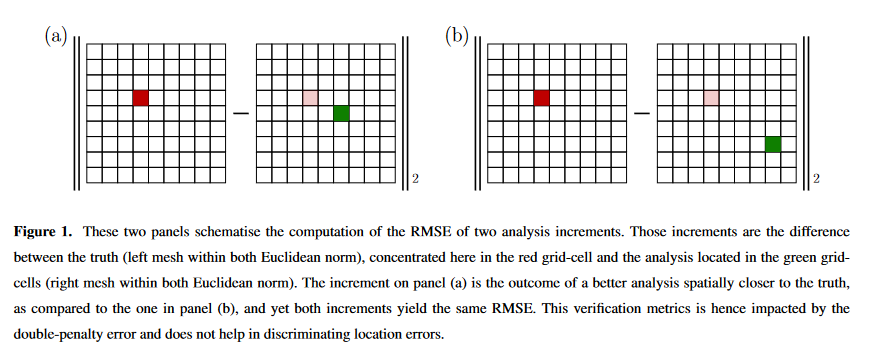
\includegraphics[width=\linewidth]{double_penalization_error.png}
    \caption{Visualisation de l'effet de double pénalisation.}
    \label{fig:double_penalization_error}
\end{figure}

La mise à jour de la DA classique peut être limitée à l'espace des valeurs des champs, ce qui entraîne une analyse confinée aux limites d'ébauche et des observations. Ceci devient une lacune majeure lorsque le désaccord entre les observations et l'état de fond résulte d'une erreur de localisation des champs ou d'une mauvaise spécification générale de ces champs. La Figure \ref{fig:prior_field} illustre des expériences de DA classique avec des analyses bénéfiques et d'autres inutiles.

\begin{figure}[h]
    \centering
    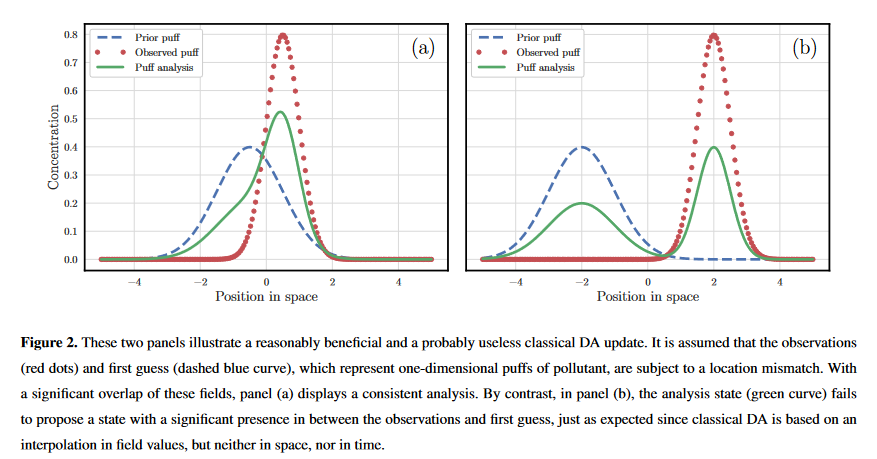
\includegraphics[width=\linewidth]{prior_field.png}
    \caption{correction avec l'approche classique à l'aide d'une norme euclidienne et celle escomptée avec une distance de type Wasserstein.}
    \label{fig:prior_field}
\end{figure}

L'objectif des approches qui vont suivre sera de présenter des méthodes d'interpolation non pas dans l'espace euclidien des intensités, mais plutôt dans un espace interpolant qui puisse prendre en compte un déplacement dans l'espace physique.

On peut considérer que l'erreur provient du choix du MSE comme mesure d'erreur, qui est une mesure localisée à une position. Une mesure plus pertinente consiste en la combinaison d'une carte de déplacement suivie de la norme classique MSE (Hoffman et al., 1995; Keil and Craig, 2009). Des métriques basées sur des approches ont pu être proposées.
Une approche élégante consiste à appliquer la théorie du \textit{transport optimal} qui est associée à la \textit{distance de Wasserstein}. Des exemples d'utilisation de l'OT peuvent être trouvés chez Farchi et al. (2016) et Vanderbecken et al. (2023).

Les travaux de thèse de Feyeux~\cite{feyeux_transport_nodate} ont permis d'utiliser une distance de Wasserstein pour l'assimilation de données issues d'images. L'article de Bocquet et al. \cite{bocquet_bridging_2023} a pour objectif de proposer une approche qui s'applique à des densités ayant des poids potentiellement différents. En effet, Feyeux fait l'hypothèse que les états sont tous dans $\mathcal P(\Omega)$, états et observations.

Si le transport optimal semble être l'approche la plus générale capable de répondre à cette problématique, on en trouve également d'autres capables de prendre en compte l'erreur de double pénalisation. En particulier, les travaux de Ravela (2007) \cite{ravela_data_2007}, la thèse de Percival (2008) ou Rosenthal (2018) \cite{rosenthal_displacement_2017}.

Les travaux de Ravela 2007 \cite{ravela_data_2007} peuvent trouver une résonance dans une approche OT via une étape d'alignement de champs puis de correction des intensités. Dans la continuité de ces travaux, Ying et al. \cite{ying_multiscale_2019, ying_improving_2023} proposent une approche multi-échelle.

On trouve des formes proches de la distance de Wasserstein en assimilation de données mais dans une toute autre perspective. Il s'agit de transporter la distribution du \textit{prior} vers celle du \textit{posterior} (El Moselhy and Marzouk, 2012; Oliver, 2014; Marzouk et al., 2017; Farchi and Bocquet, 2018; Tamang et al., 2020). On peut l'utiliser aussi pour ajuster les poids du filtre particulaire (Tamang et al., 2021, 2022). Elle a également été utilisée pour comparer des ensembles de forecast (Le Coz et al., 2023; Lledó et al., 2023), ou de précipitation (Duc and Sawada, 2023).
Aujourd'hui, on ne traite que des cas de pdf de variables aléatoires scalaires. À cause du problème du fléau de la dimension.
Dans notre cas, on traite des états qui sont des champs, pas la pdf d'une seule variable. Dans les cas de champs de dimension 2 ou 3.

Un travail de W. Steven Rosenthal \cite{rosenthal_displacement_2017} trouve des similarités avec notre problématique de vortex avec la recherche d'une fonction de courant pour pouvoir imposer un champ de déplacement incompressible. Ces travaux s'inspirent en partie de la thèse de Percival à l'université de Reading. Tout comme les travaux de Ravela, l'objectif est de corriger l'ébauche avec une transformation qui conserve les volumes. En fait, c'est une condition qui a été soulevée dans Percival 2008 et qui me semble trouver son sens en théorie du réarrangement et dans la théorie dynamique du transport optimal formulée par Bénamou (voir chapitre 7 de \cite{peyre_computational_2020} et le chapitre 2 de \cite{feyeux_transport_nodate}).

\section{Bocquet, Marc et al., Bridging classical data assimilation and optimal transport, 2023}


Posons quelques notations pour le transport optimal. Le problème consiste à trouver le plan au coût minimal transportant la mesure $\rho_0$ à $\rho_1$. Les mesures sont donc non négatives et ont une intégrale de 1. Un choix d'intégrale peut également être fait. De plus, des généralisations pour des masses différentes ont également été réalisées.

On définit un coût pour tout couple de points $(x,y) \in \Omega^2$, généralement fonction de la distance. On présente souvent le coût quadratique

$$
    \mathcal C_{bo}(x,y) = \norm{x-y}^2.
$$

On introduit l'ensemble des plans de transformations différentiables admissibles $T$

$$
    \mathcal U_{bo} = \{T:\Omega \mapsto \Omega, \quad \rho_0 = |\partial_x T|~\rho_b \circ T\},
$$où $|\partial_x T|$ est le déterminant de la jacobienne de $T$ qui prend compte de la déformation de la mesure par la conservation totale de la masse.

On peut alors définir le carré de la distance de \textit{Wasserstein} comme

$$
    \mathcal{W}^2_{\mathcal{C}_{bo}}(\rho_0, \rho_1) = \min_{T \in \mathcal U_{bo}} \int_{\Omega} \mathcal C_{bo}(x,T(x)) \rho_0(x)dx,
$$
Dont le but est de minimiser le coût total de transport d'une mesure à l'autre. D'un point de vue pratique, il n'est pas possible de résoudre le problème formulé avec un plan de transport déterministe comme énoncé par Monge. Kantorovich introduit une formulation probabiliste au XX$^{\text{e}}$ siècle. Le plan de transport est remplacé par une mesure de probabilité $\pi$ définie sur $\Omega \times \Omega$.

L'espace des transformations admissibles devient

$$
    \mathcal V_{bo} = \{\pi : \Omega \times \Omega \mapsto \mathbb R^+, \quad \rho_o(x) = \int_\Omega \pi(x, y) dy, \quad \rho_b(y) = \int_\Omega \pi(x, y) dx\}.
$$

La distance de Wasserstein au carré devient alors

$$
    \mathcal{W}^2_{\mathcal{C}_{bo}}(\rho_0, \rho_1) = \min_{T \in \mathcal V_{bo}} \int_{\Omega \times \Omega} \mathcal C_{bo}(x,y) \pi(x, y)~dxdy.
$$

Le papier actuel se focalise sur l'utilisation de la distance de Wasserstein lors de la formulation variationnelle de l'analyse.


On part ici de la fonction de coût du 3D-Var (avec la distance Euclidenne)

$$
    \mathcal J_{cl}(\bx^a) = \norm{\by^b - \bx^a}_2^2 + \norm{\by^o - \bH \bx^a}_2^2,
$$

où $\by^b$ est la prédiction du forcast, où $\by^o$ est le vecteur des observations.
En substituant la norme Euclidienne par la norme de Wasserstein on obtient la fonction de coût suivante

$$
    \mathcal J_{w}(\bx^a) = \mathcal W_2^2(\bm y^b, \bx^a) +  \mathcal W_2^2(\bm y^0, \bH \bx^a).
$$

Il est nécessaire d'équilibre les deux distances. On appelle l'état d'analyse le \textit{barycentre de Wasserstein}.

Il remarque dans les travaux de Feyeux~\cite{feyeux_transport_nodate} que cette formulation peut être inconsistent. Dans le cas où l'état est complètement observé ($\bH$ est l'identité), l'assimilation se déroule sans encombre.
La principale raison à cela est de supposer que les densités d'origine et objectif ont la même masse. Ce qui s'applique pour les deux termes de calcul de distance de Wasserstein, à la fois que $m(\bx^a) = m(\by^b)$ et $m(\bH \bx^a) = m(\by^o)$. En supposant finalement que $m(\by^b) = m(\by^o)$, l'égalité $m(\bx^a)=m(\bH \bx^a)$ est difficilement atteignable pour $\bx^a \in \mathbb R^{N_a} \setminus \text{ker}(\bH)$.
Il faut pour cela proposer une méthode qui puissent s’accommoder d'avoir des densités de masses différentes. Une résolution a été proposée dans la communauté statistique par Chizat et al. (2018). Ici une solution orientée DA.

\begin{figure}[h]
    \centering
    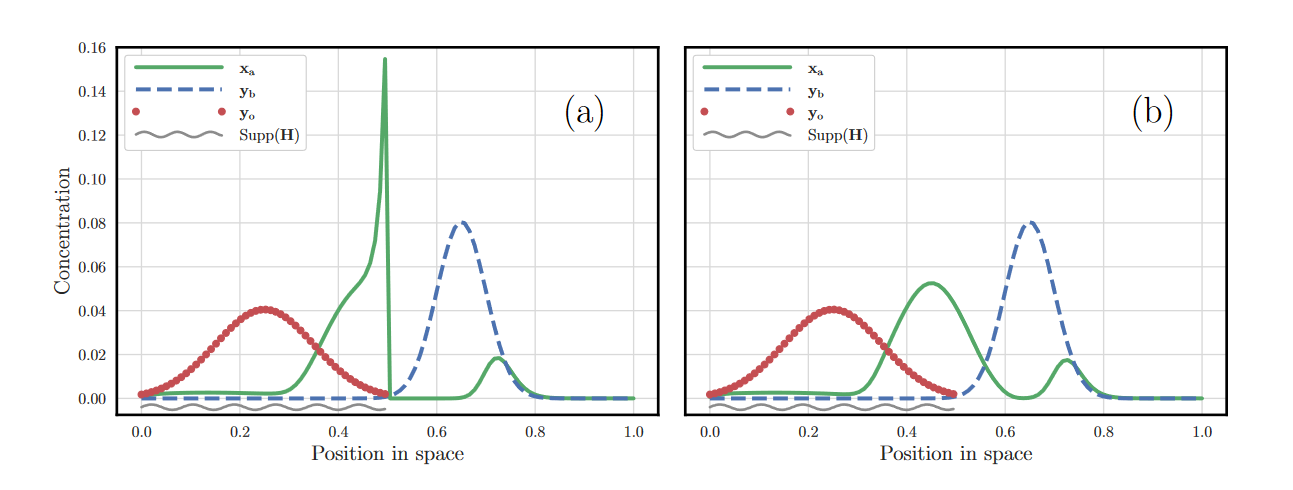
\includegraphics[width=\linewidth]{unbalanced_otda.png}
    \caption{Cas où le support n'est pas défini sur l'ensemble du domaine. Afin de conserver la masse, la solution va créer un pic d'intensité à la frontière. On souhaite un comportement comme à droite.}
    \label{fig:unbalance_otda}
\end{figure}

\subsection{Proposition}

Hypothèses: champs physiques non-négatifs, mais pas nécessairement l'ébauche et l'observation et $H$ est supposé linéaire.

Ils ont introduit l'équation (18) dans leur papier qui est une nouvelle fonction coût

$$
    L_w(\bx^a) = \min_{\bx^b \in \mathcal O_{N_b}^+, \bx^o \in \mathcal O_{N_o}^+} \{\zeta_b(\by^b - \bx^b) + \zeta_o(\by^o - \bH \bx^o) +W_{\bC_{ba}}(\bx^b, \bx^a) + W_{\bC_{oa}}(\bx^o, \bx^a)\}.
$$

Elle introduit en fait deux nouvelles variables d'optimisation $\bx^b$ et $\bx^o$. L'objectif est de pouvoir équilibre toutes les densités.
Cette fonction doit être minimisé en fonction de $\bx^b, \bx^a, \bx^o$, ses trois quantités étant libres.
Pour cela, les auteurs présente la forme duale du problème. Cette formulation duale du problème complet est assez lourde et nécessite de déterminer un plan de transport entre les trois densités. En introduisant des multiplicateurs de Lagrange, en faisant permuter les variable à minimiser ou maximiser, on obtient finalement un problème à deux variables duales à minimiser sur un polyhèdre.

$$
    \mathcal L^* = \max_{(\bbf_b,\bbf_o) \in \mathcal{U}_{bo}(\bC_{ba},\bC_{ba}, \bH)} \left\{\bbf_b^T \by^b + \bbf_o^T \by^o - \norm{\bbf_b}^2_{\bB} - \norm{\bbf_b}^2_{\bR} \right\}
$$

où $\mathcal{U}_{bo}(\bC_{ba},\bC_{ba}, \bH)$ est l'espace admissible tel  que

$$
    \mathcal{U}_{bo}(\bC_{ba},\bC_{ba}, \bH)  = \left\{ \bbf_b, \bbf_o : \forall i, j, k, \quad f^i_b + f^l_o H_l^j \leq C_{ba}^{ik} + C_{oa}^jk \right\}
$$

Il présente qq simplification mais on comprends que ce problème doit être résolue en plusieurs étapes.
Pour cela, il propose deux méthodes. Une première qui va permettre d'estimer le plan $\bP^{bo}$ à l'aide d'une régularisation entropique (via la divergence $\mathcal{KL}$). La solution assimilée est ensuite le barycentre, c'est à dire l'interpolant au sens de McCann. Ainsi $\bx^a$ est un interpolant sur la géodésique entre $\bx^o$ et $\bx^b$ dans un espace de Riemann.

Il propose une autre formulation plus directe par la suite. (Note: Je ne pense pas cette dernière soit la plus applicable à notre cas de simulation sans maillage).

La résolution se base sur les méthodes dites \textit{Smooth Optimal Transport} et des développement des termes de régularisations duaux comme dans \cite{blondel_smooth_2018}.


\subsection{Première méthode}
Pour la résolution, il introduit une régularisation entropique avec la divergence $\mathcal{KL}$. Cette régularisation permet de convexifier le problème et permet surtout d'avoir des densités $\bx^b, \bx^o$ de masse différente de 1. A noté que $\bx^b, \bx^o$ seront de même masse.

On rappelle que la définition de $\mathcal{KL}$ pour deux distributions quelconque $\bm{p}, \bm{q}$

$$
    \mathcal{KL}(\bm{p}||\bm{q}) = \sum_i p_i - \ln{\frac{p_i}{q_i}} - p_i - q_i .
$$

Le problème primal se simplifie et devient
$$
    L = \min_{\bx^b \in \mathcal O_{N_b}^+, \bx^o \in \mathcal O_{N_o}^+} \{\zeta_b(\by^b - \bx^b) + \zeta_o(\by^o - \bH \bx^o) + W_{\bC_{bo}}(\bx^b,\bx^o)\}.
$$

En ajoutant le terme de régularisation

$$
    L_\varepsilon(\bx^a) = \min_{\bx^b \in \mathcal O_{N_b}^+, \bx^o \in \mathcal O_{N_o}^+} \{\zeta_b(\by^b - \bx^b) + \zeta_o(\by^o - \bH \bx^o) + \min_{\bP \in \mathcal U_{bo}} \left(\Tr(\bC_{bo} \bP^{bo}) + \varepsilon \mathcal{KL(\bP || \bnu)}\right) \}.
$$

Le problème dépend donc de deux paramètres supplémentaires $\varepsilon > 0$ et $\bnu$. $\mathcal U_{bo}$ est l'espace admissible des plans de transfert entre $\bx^b$ et $\bx^o$. $\bnu$ est un plan de transport a priori. Or il ne peut pas être choisi à partir de $\mathcal{U}_{bo}$ celui-ci n'étant pas connu. Ainsi ils ont décidé de le choisir constant en utilisant un prior indépendant $\bx^b$ et $\bx^o$.

On peut retrouver la formule dual en équation (30) du papier mais finalement, par optimisation , on peut obtenir deux variables duals $\bbf_b, \bbf_o$ qui permettent d'obtenir le plan $\bP$.

Ainsi, en récupérant les marginales, on obtient

$$
    \bx^b = P \bm{1}_o \quad \bx^o = P^T \bm{1}_b.
$$

L'étape suivante est finalement de trouver le barycentre au sens de la distance de Wasserstein, ce qui signifie résoudre

$$
    J = \min_{\bx^a \in \mathcal O^+_{N_a}} \left\{W_{\bC_{ba}}(\bx^b, \bx^a) + W_{\bC_{oa}}(\bx^o, \bx^a)\right\}.
$$

Et cette étape offre de nombreuses variantes dans la littérature. Par exemple, l'article de Cuturi \cite{cuturi_fast_2014} offre des développements pour calculer le barycentre sur un espace de distribution empirique en faisant varier alternativement le support et les intensités des atomes. Les travaux de Feyeux \cite{feyeux_transport_nodate} offrent également de nombreuses manières de différencier et de minimiser cette fonctionnelle. En particulier, il présente les différentes dérivées pour la distance de Wasserstein.
Finalement, on se place dans le cadre d'une fonctionnelle à minimiser suivant un espace de paramètres donné et on pourra s'inspirer du chapitre 7 de \cite{peyre_computational_2020}. Ainsi, dans ce chapitre, Peyré conseille aussi d'utiliser la différentiation automatique.

\subsection{Deuxième méthode}

Pour résoudre le problème, Boucquet propose finalement une version simplifiée. On ne se base que sur deux transferts différents $\bP^{ba}, \bP^{oa}$.
On régularise pour obtenir

\begin{eqnarray*}
    \min_{\bx^b \in \mathcal O_{N_b}^+, \bx^o \in \mathcal O_{N_o}^+, \bx^a \in \mathcal O_{N_a}^+} [\zeta_b(\by^b - \bx^b) + \zeta_o(\by^o - \bH \bx^o) + W_{\bC_{ba}}(\bx^b, \bx^a) + W_{\bC_{oa}}(\bx^o, \bx^a) \\
        + \min_{\bP^{ba} \in \mathcal{U}_ba, \bP^{oa} \in \mathcal{U}_oa} \{\varepsilon \mathcal K (\bP^{oa}|\bv^{oa}) + \varepsilon \mathcal K (\bP^{ba}|\bv^{ba}) + \Tr(\bC_{oa}^T \bP^{oa}) + \Tr(\bC_{ba}^T \bP^{ba})\}].
\end{eqnarray*}


La résolution va directement prendre en compte le fait que $x_a$ est le Barycentre et par minimisation selon une variable, on retrouve une fonctionnelle à minimiser avec seulement deux variable duales à partir desquelles on peut retrouver $x_a$.

\section{Ravela et al., Data assimilation by field alignment}

Une méthode pour tenir compte des erreurs de position en appliquant un déplacement à imposer. La méthode est réalisée en deux étapes. D'abord, la détermination d'un champ de déplacement, puis la correction des intensités. L'avantage de cette méthode est qu'elle est adaptable à de nombreux filtres, en particulier les filtres d'ensemble. En effet, la seconde étape s'apparente à un filtre classique.

Il présente tout d'abord en quoi la formulation classique dans un problème de position entraîne une inflation de la matrice de covariance. La matrice issue de la perturbation d'une translation $\lambda$ devient: $C_{\lambda} = C_{XX} + \sigma^2_{\lambda} C_{\Delta\Delta}$ où $\Delta$ est la déviation du gradient (8).

Pour réaliser l'alignement, on part de la formule de Bayes comme pour les filtres d'intensité. Cependant, on introduit une nouvelle variable spatiale $\bq$ vecteur de déplacement. Dans leur travail l'état est défini sur une grille dont les positions sont $\br$. L'état est donc défini par les valeurs du champ $X = X(\br)$.

On défini $\bq$ sur la même grille tel que $X(\br  - \bq)$ est le déplacement de X par $\bq$.

On réécrit la formule de Bayes en introduisant cette nouvelle variable

$$
    P(X, \bq \mid Y) \propto P(Y \mid X, \bq) P(X^f \mid \bq) P(\bq)
$$

La Likelihood $P(Y \mid X, \bq)$ est similaire à la likelihood sur les intensités mais en appliquant au préalable le déplacement de telle sorte que les observations sont conditionnées par $X(\br - \bq)$.

On suppose donc que $Y = H(X(\br - \bq)) + \bm{\eta} \sim \mathcal{N}(0, R)$, où les observations restent bien fixes.

De même le prior sur l'intensité est inchangé en considérant au préalable la transformation $\bq$. Mais il faut remarquer que la matrice de covariance est dépendante de $\bq$. Dans un cas de filtre d'ensemble il s'agit de calculer la matrice également après transformation.

Finalement, le prior sur le déplacement $P(\mathbf{q})$ est un élément additionnel. Pour cela, on introduit une fonction d'énergie qui va régulariser les déplacements. C'est elle qui introduit un coût de déplacement. On peut penser au champ de déplacement comme à un champ d'écoulement lissé. Cette propriété de lissage amène donc à considérer des pénalisations de Tikhonov qui vont pénaliser à la fois le gradient et la divergence. Mais on peut tout à fait modifier notre a priori sur la distribution de $\mathbf{q}$. La prendre uniforme n'apporterait pas d'information, la prendre gaussienne demande de définir une manière appropriée pour la définir. La contrainte ici reste locale, mais elle introduit une forte régularité par pénalisation.

En prenant l'opposée de la log likelihood on obtient la fonction de coût associée $J(X, \bq)$. On remarquera que un terme inhabituel lié à la dépendance de $P$ à $\bq$. On note par la suite $\bp = \br - \bq$ où $\br$ est la coordonnées dans l'espace non déformé.

Ainsi on obtient

$$
    J_2(X, \bq) = \frac12 \norm{(X - X^f)(\br - \bq)}^2_{P(\bq)} + \frac12 \norm{Y - H(X(\br - \bq))}^2_{R} + L(\bq) + \frac12 \ln{|B(\bq)|}.
$$

Pour résoudre le problème on a besoin de $P(\bq)$ et dériver toute la fonction coût. On peut utiliser pour cela un ensemble comme en EnKF pour l'estimer.
Pour cela on suppose connu les déplacements associés  à chacun des membres $\bq_s$. On note $\bp_s = \br_s - \bq_s$. et on estime donc $B_Q$. Finalement, on finit par avoir une version Hybrid de la fonction de coût.

Il choisis également de fixer les déplacement dans l'évaluation de $B_Q$ pour éviter de devoir les différentier et modifier dans la version itérative. Il peut ainsi définir les gradients en fonction de $\bq_s$.

Une autre proposition consiste à séparer la phase d'alignement et de correction des intensités, c'est la méthode séquentielle. Pour cela, à partir de la fonction de cout, on écrit les équation d'Euler-Lagrange. On écrit la fonction de coût différentiée selon $\bq$ puis selon $\bX$. Je note implicitement $s$ en indice car cela est réalisé parallèlement sur l'ensemble.


\begin{eqnarray*}
    \frac{\partial J_s}{\partial \bq} = (\nabla X \mid_{\bp} - \nabla X^f \mid_{\bp})^T B_Q^{-1} (X(\bp) - X^f(\bp)) + \nabla X \mid_{\bp} H^T R^{-1} (H X(\bp) - Y) + \frac{\partial L}{\partial \bq} = 0 \\
    \frac{\partial J_s}{\partial X} =  B_Q^{-1}  (X(\bp) - X(\bp)) + H^T R^{-1} (H X(\bp) - Y) = 0.
\end{eqnarray*}

On commence par fixer $X$ à $X^f$ dans la première équation, ainsi que $Q$ ce qui permet d'obtenir

$$
    \frac{\partial L}{\partial \bq} + \nabla X \mid_{\bp} H^T R^{-1} (H X(\bp) - Y) = 0
$$

Le choix de pénaliser la divergence de $\mathbf{q}$ permet d'obtenir une équation de Poisson à résoudre avec un terme source non linéaire. Il propose de résoudre cela avec une méthode de type BFGS. Après des essais en utilisant l'autodifférentiation, je constate que ce sont des problèmes fortement non linéaires. Dans la littérature, une approche multiéchelle de cette méthode a été proposée. De cette manière, le déplacement appliqué est une composition de modes avec plus ou moins de raffinement. Selon moi, cela devrait améliorer la convergence.

Finalement, la deuxième étape consiste à résoudre la seconde équation avec $\mathbf{q}$ fixé. On peut réévaluer $B_Q$. On remarque que l'on obtient la même mise à jour qu'avec un filtre de Kalman. Avec la formule de Sherman-Morrison-Woodbury, on obtient la correction de l'intensité $\mathbf{X}$ comme combinaison linéaire du forecast et de l'innovation.

\section{Rosenthal et al., Displacement data assimilation}
Dans cet article les auteurs décide de corriger l'ébauche. Il parte de l'évaluation de l'erreur classique pour un champ de vorticité $\omega$ et il cherche $\omega_a$ qui minimise

Ainsi, il part de l'idée de résoudre 2 fonctions coût à la suite, une pour corriger la position (champ de déplacement paramétré par $a$) et l'autre qui va corriger le l'ébauche qui aura été déplacé. On retrouve ainsi la même démarche que Ravela.

\begin{eqnarray*}
    \mathcal J_p(a) = \frac12 \norm{d - h_a(a)}^2_{R^{-1}} + \frac12 \norm{a - a^f}_{P^{-1}_{a}}, \\
    \mathcal J_a(\omega) = \frac12 \norm{d - h(\omega)}^2_{R^{-1}} + \frac12 \norm{\omega - \omega^f}_{P^{-1}_{\omega}},
\end{eqnarray*}~avec $d$ les observations et $R^{-1}$ la matrice de covariance sur les observations qui sont utilisées plusieurs fois. Les opérateurs d'observations sont différents (uniquement déterminant pour la différentiation), ainsi que les statistiques sur les déplacements $a^f$ et $P_{a}$.

La première chose qui est réalisée est de définir une transformation. Il définit pour cela un mappage entre les variables dans l'espace déformé $Z$ et dans l'espace non déformé $z$ (j'ai l'impression que la convention est inversée...). Les coordonnées $Z$ permettent ensuite d'évaluer l'erreur avec la ground truth ou d'évaluer la prédiction des observations. Par exemple, pour le cas où le champ est directement observé sur une discrétisation eulérienne.

$$
    J_a(\omega) = \norm{\omega^t(Z) - \omega(Z)}^2
$$

En définissant une transformation inversible $Z = \Phi(z; a)$, on peut ensuite appliquer la transformation pour obtenir le champ déplacé de $\omega^f$ défini avec $z$

$$
    J_p(a) = \frac12 \norm{\omega^t(Z) - \omega^f \circ \Phi^{-1}(Z;a)}^2.
$$

Quel est donc cette transformation ? Elle doit respecter la conservation de la vorticité totale. Plutôt qu'une transformation canonique qui à le problème d'être implicite. Ici, il propose d'intégrer la fonction de courant sur un interval de temps fixe.
Ainsi $\Phi$ devient

$$
    \Phi(x,y;a) = (x, y) + \int_0^1 \left(-\Psi_y[x(t),y(t); a], \Psi_x[x(t), y(t); a]\right)dt.
$$

On choisie alors de paramétrer la fonction courant $\Psi$ linéairement avec $a$ par exemple $\Psi(x,y; a) = B a$. L'inverse de la transformation est alors obtenue en substituant les coordonnées et en prenant $a \mapsto -a$. Comme cette hypothèse se base sur de petite transformation, on pourra donc trouver des séquence de $(a_{t_i})_{i=1}^{n}$ pour pouvoir faire l'intégration.

En ce qui concerne la régularisation de $a$, il propose simplement de faire de la propagation de $P_{\omega}$. Il suffit pour cela de connaitre $T_{\omega a}$ ainsi que son (pseudo)inverse $T{a \omega}$ ce qui donne $P_a = T_{a \omega} P_{\omega} T_{\omega a}$. Dans le cas où $P_{\omega}$ n'est pas connu, on peut faire de la régularisation sur la déformation. Toutefois, il signale que $P_a$ peut ne plus être SDP. Ainsi, une étape de projection est nécessaire.

Mais, l'utilisation d'un ensemble permet de régler ce souci. En effet, Pour un ensemble $X^f$ de forecast, on peut approximer $P_a$ comme

$$
    P_a = \frac{1}{N-1} [T_{a \omega}(X - \bar x \bm{11}^T)]^T [T_{a \omega}(X - \bar x \bm{11}^T)]
$$

En utilisant l'approximation tangentiel de l'opérateur $h_p$ qui relie les paramètres $a$ de déformation et les prédictions, on peut obtenir alors la correction sur les positions $A = {a_j}_{j=1}^{N_{ens}}$

\begin{equation*}
    A = L \left[ d_V - h_a(X^f)\right],
\end{equation*}~où $L$ est défini comme $L = P_a H^T (R + H_p P_a H_p^T)$ avec $H_p$ la linéarisation de l'opérateur d'observation en fonction de $a$ autour de $0$ \footnote{Il y a une erreur (il me semble) dans leur article}

\begin{eqnarray*}
    H_p &=& \nabla_a h_p \left(A; X^f\right) \\
    &=& \nabla_a h_a(X^f \circ \Phi^{-1}(Z; A)) \\
    &=& \nabla_\omega h_a(X \circ \Phi^{-1}) \cdot \nabla_a [X \circ \Phi^{-1}(Z;A)] \\
    &=& \nabla_\omega h_a(X \circ \Phi^{-1}) \cdot \nabla_z (X\circ \Phi^{-1}(Z;A)) \cdot \nabla_a \Phi^{-1} (Z; A).
\end{eqnarray*}~avec

\begin{equation*}
    \nabla_a \Phi^{-1}(Z;A) = \nabla_a \Phi(Z;-A) = \left[B_y(Z) , -B_x(Z)\right]^T.
\end{equation*}

Il propose d'appliquer plusieurs cette correction, mais il ne précise pas le nombre de fois à mon avis cela est arbitraire et correspond à l'intégration dans le temps de la fonction de courant ?

Ainsi dans cet article, il propose une correction qui vérifie des contrainte physique (\textit{divergence-free}). La régularisation sur le déplacement avec un prior doit être pris en compte et en pratique il préfère utiliser une régularisation de type Thikhonov sur les déformations.

\section{Notes personnelles}

Quelques remarques personnelles sur ces trois développements

\begin{itemize}
    \item Ravela 2007 \cite{ravela_data_2007} : Les travaux de Ravela sont intéressants dans le sens où ils peuvent être combinés avec des méthodes classiques en assimilation de données. Néanmoins, la correction de position est basée sur un problème de minimisation non linéaire. Dans les tests que j'ai pu réaliser pour l'étape d'alignement, j'ai pu constater que la solution reste souvent dans des minima locaux. De plus, il y a une étape de calibration des hyperparamètres pour la régularisation. Si cela est mal réalisé, on se retrouve facilement avec des champs de déplacement qui ne sont pas réguliers. Dans notre cas de simulations sans maillage, on peut potentiellement utiliser la même méthode sur une grille régulière pour obtenir $\mathbf{q}$ puis appliquer par interpolation la déformation. L'étape qui suit serait la même qu'auparavant, c'est-à-dire corriger les intensités. Cependant, on peut espérer avoir une discrétisation plus cohérente avec la solution analysée.
    \item Rosenthal 2017 \cite{rosenthal_displacement_2017} : Dans cet article, l'objectif est similaire à celui de Ravela, c'est-à-dire de modifier l'ébauche pour réduire l'erreur avec les données. Ici, la transformation appliquée doit être incompressible. Ainsi, ils vont chercher à déterminer les paramètres d'une fonction de courant qui est ensuite intégrée pour mettre à jour l'ébauche. Pour notre cas de méthode particulaire, cet article présentant des mises à jour de l'ébauche est intéressant. L'intérêt ici par rapport à l'article de Ravela est que le transport se fait de manière physiquement consistante. L'application pour la méthode VIC que j'utilise peut être assez proche ici. On appliquerait la fonction courant déterminée sur les particules de l'ébauche, mettant à jour l'ensemble d'ébauche. Puis, en travaillant sur l'ensemble transporté, on applique également les filtres d'ensemble classiques (Part-EnKF par exemple). Pour un cas plus général, par exemple en mécanique des solides avec la méthode MPM ou DEM, pourrait-on imaginer utiliser le même type de transformation ? En MPM, on peut imaginer appliquer une transformation, tout comme en VIC, les points matériau peuvent être facilement déplacés, à voir sur les conditions d'admissibilité cinématique. Pour la DEM, cela est plus complexe. En effet, les contraintes sur la mise à jour concernent la position des particules les unes par rapport aux autres. Ainsi, la mise à jour se fait par la détermination d'une force qui va être régularisée sur les interpénétrations et intégrée dans le schéma temporel. Pourrait-on imaginer réaliser une correction de cette force pour pouvoir modifier la trajectoire des particules sur un intervalle de temps fixe ?
    \item Bocquet 2023  \cite{bocquet_bridging_2023} :Cet article propose une méthode qui applique le transport optimal à l'assimilation de données en introduisant deux champs supplémentaires pour traiter des cas où les masses de densité diffèrent. L'objectif est de travailler avec des observations partielles de champs et des observations bruitées, en corrigeant à la fois la position et les poids dans un espace de Riemann associé à la distance de Wasserstein. Ici, le choix est fait de travailler sur des discrétisations eulériennes pour définir les états $\bx^b, \bx^o, \bx^a$. Dans l'article les discrétisation des états $\bx$ sont toutes les mêmes. Dans notre applications aux méthodes sans maillage, on connait la discrétisation de $\bx^b$ uniquement. Cette article travaille sur des discrétisation de densité de champ, ainsi il me semble possible de pouvoir travailler directement sur les distributions \textit{empiriques} de particules c'est dire $P_i = \sum_{p} \Gamma_p \delta_{z_p}$. Pour définir la discrétisation de $\bx^o$, on pourrait choisir une discrétisation régulière arbitraire. En effet, il faudrait éviter de prendre uniquement le support des observations, le risque étant d'avoir un déséquilibre de masse. Finalement, l'étape de barycentre pourrait être obtenu par minimisation d'une fonction coût de type $L(\bx) = W(\bx^o, x) + W(\bx^b, \bx)$, en partant d'une discrétisation Lagrangienne du champ (par exemple en partant de $\bx^b$) et minimiser alternativement en fonction de $z^p$ et $\Gamma^p$. L'objectif étant de suivre au mieux la géodésic. On pourrait s'inspirer des travaux de Cuturi et al. \cite{cuturi_fast_2014} ou bien de proposer une méthode de minimisation par gradient flow par exemple \cite{liutkus_sliced-wasserstein_2019}. La formulation dynamique du problème de transport optimal pourrait être interessante aussi car elle permet de déterminer un champ de vitesse, mais je ne crois pas encore avoir acquis l'ensemble des subtilités dans ce cas (voir chapitre 7 de \cite{peyre_computational_2020}). Egalement je viens de trouver des formulations de MPM qui mêle MPM et OT \cite{li_optimal_2010}.
\end{itemize}


\bibliography{C:/Users/md266594/mar-dvd-thesis/biblio.bib}

\end{document}